\documentclass[journal]{IEEEtran}
\IEEEoverridecommandlockouts

\usepackage{textcase}
\usepackage{changes}
\usepackage{gensymb}
\usepackage{cite}
\usepackage{amsmath,amssymb,amsfonts}
\usepackage{algorithmic}
\usepackage{textcomp}
\usepackage{graphicx}
%\usepackage{citesort}
\usepackage{amsthm}			% 自定义环境样式包
\usepackage{amssymb}
\usepackage{amsfonts}
\usepackage{amsmath}
\usepackage{epsfig}
\usepackage{color}
\usepackage{fancybox}
\usepackage{textcomp}
\usepackage{multirow}
\usepackage{makecell}       % multiple lines inside a cell of a table
\usepackage{setspa ce}
\usepackage{psfrag}
\usepackage{booktabs}
\usepackage{float}
\usepackage{caption}
\usepackage{subcaption}
\usepackage{placeins}
%\floatstyle{plaintop}
\restylefloat{table}
\usepackage{tablefootnote}
%\usepackage{caption}
%\usepackage[caption = false]{subfig}
\usepackage[ruled]{algorithm2e}
\renewcommand{\algorithmcfname}{Algorithm}
\SetKwInput{KwData}{\textbf{Initialization}}
\usepackage{mathrsfs}
\newcommand{\blue}[1]{{\textcolor[rgb]{0,0,1}{#1}}}
\newcommand{\red}[1]{{\textcolor[rgb]{1,0,0}{#1}}}
\newtheorem{Lemma}{Lemma}
\newtheorem{Theorem}{Theorem}
\newtheorem{Remark}{Remark}
\newcommand{\CLASSINPUTtoptextmargin}{2.4cm}
\input macro
\def\BibTeX{{\rm B\kern-.05em{\sc i\kern-.025em b}\kern-.08em
    T\kern-.1667em\lower.7ex\hbox{E}\kern-.125emX}}

%% 自定义包
\usepackage{svg} 								% 支持SVG图片
\usepackage{bm}									%
\usepackage{enumitem}							% item支持更多格式
\usepackage[numbers,sort&compress]{natbib}		% 文献引用连号时[1,2,3]变成[1-3]
\usepackage{breqn}								% 公式过长自动换行

%% 自定义字符
\newcommand{\T}{^{\mathrm{T}}} % 转置
\newcommand{\HT}{^{\mathrm{H}}} % 共轭转置
\newcommand{\diag}{{\sf diag}} % 生成对角矩阵
\newcommand{\off}{{\sf off}} % 对角元素置0
\newcommand{\vect}{{\sf vec}} % 向量化

%% 自定义环境样式
\renewcommand{\proofname}{\textit{Proof:}}

% 覆盖 breqn 的编号设置
\renewcommand{\theequation}{\arabic{equation}}

% set the img folder
\graphicspath{{img/}}
    
\begin{document}

\title{Learning-Aided Joint Channel Estimation and Detection in OTFS with Graph Neural Networks}

\author{Xinwei Qu}

\maketitle

\begin{abstract}


\end{abstract}

\begin{IEEEkeywords}
OTFS joint channel estimation and symbol detection, graph neural network, 6G
\end{IEEEkeywords}

\section{Introduction}
% todo
% (NN)
% (GNN)
% OTFS
% OFDM
% VB

\subsection{Related Works}

\subsection{Contributions}
The main contributions of this paper are summarized as follows.
\begin{itemize}
% 2
\item we propose an OTFS frame design that increase the transmission efficiency and overcomes the overspreading channel issue
% 1
\item We propose a novel neural network-based framework for joint channel estimation and symbol detection for OTFS systems, referred as Joint Parallel Interference Cancellation Network (JPICNet) framework. The proposed framework integrates the joint PIC scheme and graph neural network. 
% 3
\item we incorporate attention mechanism into neural network-based framework to improve the performance.
\end{itemize}

\subsection{Notations}
$a$, $\mathbf a$ and $\mathbf A$ demote scalar, vector, and matrix respectively. $\mathbf  I$ denotes an identity matrix. $\mathbb{C}^{M\times N}$ denotes the set of $M\times N$ dimensional complex matrix. $(\cdot)\T$, $(\cdot)\HT$, $(\cdot)^*$, and $[\cdot]_M$ represent the transpose, Hermitian transpose, conjugate, and mod-$M$ operations. $\odot$ denotes Hadamard multiplication. $\diag(\bm a)$ denotes the operation to diagonize a vector $\bm a$, $\off(\mathbf A)$ forces all diagonal elements to zero. We define $\mathbf a=\vect(\mathbf A)$ as the column-wise vectorization of matrix $\mathbf A$. For any real number, $\lfloor \cdot \rfloor$ denotes the greatest integer less than or equal.

\section{System Model}
% todo
% Xp, x_p, k_p, {l_p}_0, ..., {l_p}_last


We first introduce the OTFS mod/demod and its frame structure. Subsequently, we derive the input-output relation in the delay-Doppler (DD) domain for the two most widely adopted pulse-shaping waveforms.


\subsection{OTFS System}
\begin{figure*}[!t]
  \centering
  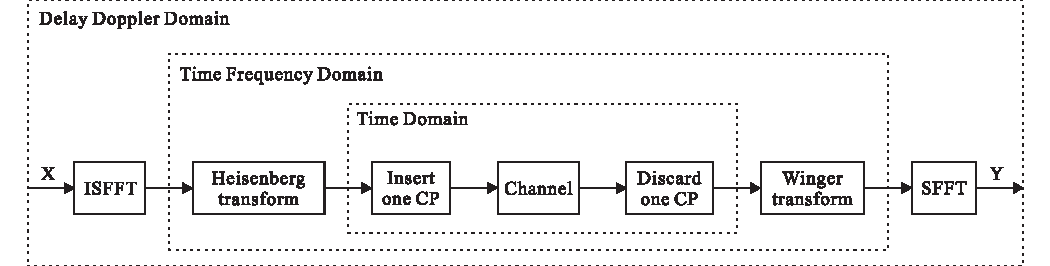
\includegraphics[scale=1]{otfs_sys.pdf}
  \caption{OTFS mode/demod}
  \label{fig:otfs-sys}
\end{figure*}
We consider a single input single output (SISO) OTFS system as illustrated in Fig.~\ref{fig:otfs-sys}. The transmitter operates an OTFS frame (detailed in \ref{sec:sys-frame}), $\mathbf X[k,l] \in \mathbb{C}^{K \times L}$, with $k = 0, \cdots, K-1$ and $l = 0, \cdots, L-1$ indexing discretized Doppler and delay shifts, respectively. After transposition. the frame is converted to the time-frequency (TF) domain via the inverse symplectic finite Fourier transform (ISFFT), mapping the data on $L\times K$ grids with uniform intervals $\Delta f$ (Hz) and $T=1/\Delta f$ (seconds).  The time-domain signal is synthesized using (discrete) Heisenberg transform with a pulse-shaping waveform employing a single initial cyclic prefix spanning the full OTFS frame duration. The time-domain signal is transmitted over a time-varying wireless channel characterized by the delay-Doppler impulse response $h(\tau, v)$ as \cite{7925924},
\begin{equation}
h(\tau, v) = \sum_{i=1}^P h_i \delta (\tau - {\tau}_i) \delta (v - v_i) ,
\end{equation}
where $\delta(\cdot)$ denotes the Dirac delta function, $h_i \sim \mathcal{N}(0, \frac{1}{P})$ is the gain of the $i$-th propagation path, and $P$ represents the total number of paths. Each path is characterized by distinct delay and/or Doppler shifts, modeling the channel response between the receiver and either moving reflectors or the transmitting source. The delay and Doppler shifts are given as,
\begin{equation}
{\tau}_i = l_i \frac{T}{L}, v_i = k_i \frac{\Delta f}{K},
\end{equation}
respectively. Let the integers $l_i \in [0, l_\max]$ and $k_i \in [-k_\max, k_\max]$ represent the delay and Doppler shift indices, respectively, where $l_\max$ and $k_\max$ denote the maximum delay index and maximum Doppler shift index across all propagation paths. Note that we restrict our consideration to integer-valued indices, as fractional delay and Doppler shifts can be equivalently represented through virtual integer taps in the delay-Doppler domain using the techniques described in \cite{6563167, 8377159, 8516353}.

At the receiver, the time-domain signal is first transformed to the time-frequency (TF) domain using a matched filter followed by Wigner transform. The resulting signal is then transposed and converted to the delay-Doppler (DD) domain through the symplectic finite Fourier transform (SFFT), producing the received frame $\mathbf{Y}[k,l] \in \mathbb{C}^{K \times L}$. The DD domain input-output relationship can be formulated in a vector form as \cite{10264119},
\begin{equation}
\mathbf y = \mathbf H\mathbf x + \mathbf z,
\label{eq:sys-DD}
\end{equation}
where $\mathbf x = \vect(\mathbf  X\T)$, $\mathbf  y = \vect(\mathbf  Y\T)$, and $\mathbf z \sim \mathcal{CN}(0, \sigma^2)$ is an independent and identically distributed (i.i.d.) Gaussian noise \cite{8516353, 10264119, 7925924}.


\subsection{OTFS Frame Structure}\label{sec:sys-frame}
\begin{figure}[htbp]
    \centering
    \includegraphics[scale=1]{otfs_frame}
    \caption{OTFS frame structure with the last pilot delay index at $l_{p,\text{last}} = (N_p - 1)(l_\max + 1)$}
    \label{fig:otfs_frame}
\end{figure}

As illustrated in Fig.~\ref{fig:otfs_frame}, a superimposed OTFS frame structure is considered, where pilot and data symbols are jointly embedded over delay-Doppler grids, i.e.,
\begin{equation}
\mathbf{X} = \mathbf{X}_d + \mathbf{X}_p,
\end{equation}
where $\mathbf X_d[k, l] \in \mathbb{C}^{K \times L}$ denotes the data frame composed of quadrature amplitude modulation (QAM) symbols drawn from a constellation $\mathcal{A}$ with average energy $E_d$. The pilot frame $\mathbf X_p[k, l]$ contains nonzero elements only at designated positions, i.e.,
\begin{equation}
\mathbf X_p[k, l] =
\begin{cases}
x_p, & k = k_p,\ l = l_p, \\
0, & \text{otherwise},
\end{cases}
\end{equation}
where $x_p$ is the pilot symbol with energy $E_p$, $k_p = \lfloor (K-1)/2 \rfloor$ is the Doppler index of all pilots, and $l_p = i(l_\max + 1)$ for $i = 0, \dots, N_p - 1$ are their delay indices. Here, $N_p = \lfloor L / (l_\max + 1) \rfloor$ denotes the total number of pilots. Each pilot facilitates channel estimation over a region of size $K \times (l_\max + 1)$ in the DD domain.



%% todo
% 解释 H 在两种Pulse的值

\section{OTFS Channel Estimation using VB}
\subsection{OTFS Channel Estimation using VB}
We assume the channel follows the Gaussian distribution, i.e.,
\begin{equation}
p(h|\gamma) = \prod_{i=0}^{P_{\max}-1}p(h_i|\gamma_i) = \prod_{i=0}^{P-1}\mathcal{CN}(h_i;0, \gamma_i^{-1}),
\end{equation}
where $P_{\max}=(l_\max+1)(2k_\max+1)$, $\gamma=[\gamma_0,\gamma_1,\cdots,\gamma_{P_{\max}-1}]$ is the precision vector of $h$. $\gamma$ follows the Gamma distribution, i.e.,
\begin{equation}
p(\gamma)=\text{Gamma}(\gamma; a, b)
\end{equation}
where $a$ is the shape parameter and $b$ is the inverse scale parameter. Also, we assume the noise obeys the Gaussian distribution, i.e.,
\begin{equation}
p(z)=\mathbf z \sim \mathcal{CN}(0, \alpha^{-1}\bm I)
\end{equation}
where $\alpha$ obeys the Gamma distribution, i.e.,
\begin{equation}
p(\alpha)=\text{Gamma}(\alpha; c, d)
\end{equation}
where $c$ is the shape parameter and $d$ is the inverse scale parameter. For all parameters, we define $\Theta=\{h,\gamma, \alpha\}$.

Here, we use the mean field assumption to estimate the channel, i.e.,
\begin{equation}
\begin{split}
p(y, \Theta) &= p(y|h,\alpha)p(h|\gamma)p(\gamma)p(\alpha) \\
lnp(y, \Theta) &= lnp(y|h,\alpha) + lnp(h|\gamma) + lnp(\gamma) + lnp(\alpha)
\end{split}
\end{equation}
Here, we use a distribution family $Q$ over $\Theta$ to approximate $p(\Theta|y)$, i.e.,
\begin{equation}
\begin{split}
p(\Theta|y) &= \mathop{\arg\min}\limits_{q(\Theta)\in Q} KL(q(\Theta) || p(\Theta|y)) \\
&= \mathop{\arg\min}\limits_{q(\Theta)\in Q} -\int_{\Theta}q(\Theta)\text{ln} \frac{p(\Theta|y)}{q(\Theta)}d\Theta
\end{split}
\end{equation}
where $q(\Theta)$ follows the mean field assumption, i.e.,
\begin{equation}
q(\Theta) = q(h)q(\gamma)q(\alpha)
\end{equation}
Therefore, we can update the probability functions as follows:
\begin{equation}
q^{(t+1)}(\alpha) \propto exp( \mathbb{E}_{q^{(t)}_{-\alpha}}[\text{ln}p(y,\Theta)] \} )
\end{equation}
\begin{equation}
q^{(t+1)}(h) \propto exp( \mathbb{E}_{q^{(t)}_{-h}}[\text{ln}p(y,\Theta)] \} )
\end{equation}
\begin{equation}
q^{(t+1)}(\gamma) \propto exp( \mathbb{E}_{q^{(t)}_{-\gamma}}[\text{ln}p(y,\Theta)] \} )
\end{equation}
The update is computed as follows
\begin{enumerate}[label=\arabic*)]
    \item Update $q(\alpha)$
    	\begin{align}
    	q^{(t+1)}(\alpha) &\propto exp( \mathbb{E}_{q^{(t)}_{-\alpha}}[\text{ln}p(y, \Theta)] \} ) \\
    	lnq^{(t+1)}(\alpha) &\propto \mathbb{E}_{q^{(t)}_{-\alpha}}[\text{ln}p(y, \Theta)] \\
    	lnq^{(t+1)}(\alpha) &\propto \mathbb{E}_{q^{(t)}_{h}}[\text{ln}p(y|h, \alpha)] + lnp(\alpha)
    	\end{align}
    	Here, 
    	\begin{align}
    	p(y|h, \alpha) &= \mathcal{CN}(\bm y_p; \bm\Phi_p\bm h, \alpha^{-1}\bm I)
    	\end{align}
    \item 2
    \item 3
\end{enumerate}


\subsection{Variational Bayes Interference}



\section{Joint Parallel Interference Cancellation Network}
% todo
% Fig.\ref{}

In this section, we propose a novel JPICNet framework that enhance the joint PIC scheme with graph neural network. Fig.\ref{} illustrates the process of the proposed framework. The proposed framework consists of channel parameters estimation (CPE), the GNN-aided symbol detection (GSD) and the GNN-aided channel estimation (GCHE) modules. CPE runs only once to generate initial input for GSD, while GSD and GCHE iteratively exchange outputs in a feedback loop.

\subsection{Channel Parameters Estimation}
% todo
% Estimation area
Estimation area $k \in [0, K-1], l \in [0, lmax]$

Based on the transmission arrangement, we can express the received signal in the channel estimation area as,
\begin{equation}
\begin{split}
y[k, l] = &h[k - k_p, l-{l_p}_0]x_p \\
& + \sum_i^P h_i \beta[k, l, k_i, l_i] x_d[[k-k_i]_K, [l-l_i]_L]\\
& + \tilde{z}[k, l].
\end{split}
\label{eq:JPICNet-CPE-rxSigCHE}
\end{equation}
%The parameter $\beta[k, l, k_i, l_i]$ corresponds to OTFS with ideal waveform is given as,
%\begin{equation}
%    \beta[k, l, k_i, l_i] = e^{-j2\pi  \frac{k_il_i}{KL}}, 
%\end{equation}
%while $\beta[k, l, k_i, l_i]$ applies to OTFS with rectangular waveform is given as,
%
%\begin{equation}
%\beta[k, l, k_i, l_i] = 
%\begin{cases}
%   	e^{j2\pi  \frac{k_i(l-l_i)}{KL}} & l_i \leq l < L, \\
%   	e^{-2j\pi \left( \frac{[k-k_i]_K}{K}\right)}e^{j2\pi \frac{k_i(l-l_i)}{KL}} & 0 	\leq l < l_i. \\
%\end{cases}
%\end{equation}
The parameter $\beta[k, l, k_i, l_i]$ has distinct forms for different OTFS waveforms:
\begin{enumerate}
	\renewcommand{\labelenumi}{\roman{enumi})} % 小写罗马数字 + 右括号
    \item \textit{Ideal waveform}:
    \begin{equation}
        \beta_{\text{ideal}}[k, l, k_i, l_i] = e^{-j2\pi \frac{k_i l_i}{KL}},
    \end{equation}
    \item \textit{Rectangular waveform}:
    \begin{equation}
    \begin{split}
        & \beta_{\text{rect}}[k, l, k_i, l_i] =  \\
        & \hspace{1em}\begin{cases}
            e^{j2\pi \frac{k_i(l-l_i)}{KL}}, & l_i \leq l < L, \\
            e^{-j2\pi \left(\frac{[k-k_i]_K}{K}\right)} e^{j2\pi \frac{k_i(l-l_i)}{KL}}, & 0 \leq l < l_i.
        \end{cases}
    \end{split}
    \end{equation}
\end{enumerate}
From \eqref{eq:JPICNet-CPE-rxSigCHE}, the second term arises from the interference between pilot and data symbols. For simplicity, this cross-interference can be modeled as an additive noise term in subsequent analysis, i.e.,
\begin{equation}
\mathcal{I}[k, l] = \sum_i^P h_i \beta[k, l, k_i, l_i] x_d[[k+k_i]_K, [l+l_i]_L].
\end{equation}
The interference term $\mathcal{I}[k, l]$ is zero-mean ($\mathbb{E}[\mathcal{I}\{[k, l]\}=0$) with its variance given by,
\begin{equation}
\text{Var}(\mathcal{I}[k, l]) = E_d.
\end{equation}
\begin{proof}
The proof is given in Appendix~\ref{app:cpe-inter-mu-var}.
\end{proof}

Based on the received signal model in \eqref{eq:JPICNet-CPE-rxSigCHE}, we propose a threshold-based channel estimation algorithm as follows. For each delay-Doppler bin $(k,l)$, if the received energy $|y[k, l]|^2$ falls below a predefined threshold $\mathcal{T}$, we declare an empty bin (no path present). Otherwise, we obtain an initial channel estimate and its variance, i.e.,
%\begin{equation}
%\hat{h}[k - k_p, l-{l_p}_0]= [|x_p|^2 + P(\sigma^2+E_d)]^{-1}x_p^*y[k,l]
%\end{equation}
\begin{subequations}
\begin{align}
\hat{h}[k - k_p, l-{l_p}_0] &= y[k,l]/x_p, \label{eq:CPE-h} \\
\hat{hv}[k - k_p, l-{l_p}_0] &= \frac{E_d + \sigma^2}{E_p}. \label{eq:CPE-hv}
\end{align}
\end{subequations}
Therefore, the threshold provides a mask vector $\mathbf h_m$ to indicate whether there is a path along the delay vector $\mathbf k$ and Doppler vector $\mathbf l$, i.e,
\begin{subequations}
\begin{align}
\mathbf  h_m = & [h_{m0}, \cdots, h_{mi}, \cdots, h_{mP_{max}}], \label{eq:CPE-hm} \\
\mathbf  k = & [-k_{max}, \cdots, 0, \cdots, k_{max}, \cdots, k_{i}, \cdots, \notag\\
&-k_{max}, \cdots, 0, \cdots, k_{max}],\label{eq:CPE-km} \\
\mathbf  l = & [0, 1, \cdots, l_{max}, \cdots, l_{i}, \cdots, 0, 1, \cdots, l_{max}]. \label{eq:CPE-lm}
\end{align}
\end{subequations}
where $h_{mi} = 1 $ denotes a path at $( k_{i}, l_{i})$ or $h_{mi} = 0$ otherwise, and $P_{max} = (l_{max}+1)(2k_{max}+1)$.


%% todo
% \hat{H}
% V_\hat{H}

\subsection{GNN-aided Symbol Detection}
We need to 

At each iteration $t$, the symbol vector $\bm{x}$ defined in \eqref{eq:sys-DD} is treated as a random vector, with its statistical parameters estimated from the observation $\bm{y}$. based on the same equation. The conditional Gaussian probability distribution function (PDF) is subsequently derived as,
\begin{equation}
p^{(t)}(\mathbf x|\mathbf y) = \mathcal{N}(\mathbf x, \bm \mu_{\mathbf x}^{(t)}; \bm\Sigma_{\mathbf x}^{(t)}),
\end{equation}
where
\begin{subequations}
\begin{align}
\bm\mu_{\mathbf x}^{(t)} =& (\mathbf  I\odot\hat{\mathbf  H}^{(t)\HT} \hat{\mathbf  H}^{(t)})^{-1}(\hat{\mathbf H}^{(t)\HT}\mathbf y - \notag\\
& \off(\hat{\mathbf  H}^{(t)\HT} \hat{\mathbf H}^{(t)})\hat{\mathbf X}^{(t-1)} - \hat{\mathbf H}^{(t)\HT} \hat{\mathbf H}^{(t)}\mathbf X_p), \label{eq:GSD-mean} \\
\bm\Sigma_{\mathbf x}^{(t)} =& (\sigma^2 + \sigma_x^2 \mathbf D_{\Delta \hat{\bm H}})(\mathbf I\odot\hat{\mathbf H}^{(t)\HT} \hat{\mathbf H}^{(t)})^{-1}. \label{eq:GSD-cov} 
\end{align}
\end{subequations}
where
\begin{equation}
\mathbf D_{\Delta \hat{\mathbf H}} = \diag(\sum_{i=0}^{KL-1}\bm \Sigma_{\hat{\mathbf H}}[:, i]),
\end{equation}
$\bm\Sigma_{\hat{\mathbf H}}$ denotes the variance matrix of $\hat{\mathbf H}$, and $\sum_{i=0}^{KL-1}\bm \Sigma_{\hat{\mathbf H}}[:, i]$ means we sum all columns of $\bm\Sigma_{\hat{\mathbf H}}$ together to build a column vector.

\begin{proof}
The proof is given in Appendix~\ref{app:GSD}.
\end{proof}

% todo
% X

\subsection{GNN-aided Channel Estimation}
Rewriting \eqref{eq:sys-DD} for channel estimation, we have
\begin{equation}
\mathbf y = \mathbf\Phi \mathbf h + \mathbf z,
\label{eq:GCHE-sys}
\end{equation}
where $\mathbf h$ is the path gain in the time domain,  
\[
\begin{split}
& \mathbf\Phi = \\
& \begin{bmatrix}
    \Phi_{k_{m0}, l_{m0}}(1, 1) & \cdots & \Phi_{k_{mP_{max}}, l_{k_{mP_{max}}}}(KL, P_{max}) \\ 
	\vdots & \ddots  & \vdots \\  
    \Phi_{k_{m0}, l_{m0}}(KL, 1) & \cdots & \Phi_{k_{mP_{max}}, l_{k_{mP_{max}}}}(KL, P_{max}) \\
\end{bmatrix},
\end{split}
\]
where $(kL+l, i)$th entry of $\mathbf\Phi \in \mathcal{C}^{(KL-1)\times P_{max}}$ is \cite{9785832},
\begin{dmath}
\Phi_{k_{mi}, l_{mi}}(kL+l, i) = X([k-k_{mi}]_K, [l-l_{mi}]_L)\beta[k, l, k_{mi}, l_{mi}].
\end{dmath}
As $\mathbf\Phi$ is unavailable, its estimate at the $t$-th iteration is employed for channel estimation, i.e.,
\begin{equation}
\begin{split}
\mathbf y &= \mathbf\Phi^{(t)} \mathbf h + \mathbf\Delta\Phi^{(t)} \mathbf h  + \mathbf z, \\
&= \mathbf\Phi^{(t)} \mathbf h + \mathbf z_2,
\end{split}
\end{equation}
where $\mathbf\Phi=\mathbf\Phi^{(t)}+\mathbf\Delta\Phi^{(t)}$ and $\mathbf z_2 = \mathbf\Delta\Phi^{(t)} \mathbf h  + \mathbf z$ is assumed to be the effective noise.


Inspired by \cite{945004, 5493831}, we implement a linear minimum-mean-squared
error (MMSE) channel estimation , i.e.,
\begin{subequations}
\begin{align}
\hat{\mathbf h}^{(t)} = & \hspace{0.3em} \mathbf R_{\mathbf h}\mathbf\Phi^{(t)\HT}(\mathbf \Phi^{(t)}\mathbf R_{\mathbf h}\mathbf\Phi^{(t)\HT}\mathbf + \notag \\
& \hspace{0.3em} \frac{1}{P} \diag(\mathbf h_m) \mathbf D_{\Delta \bm\Phi^{(t)}} +\sigma^2\mathbf I)^{-1}\mathbf y, \label{eq:GCHE-mean} \\
\text{Var}(\hat{\mathbf h}^{(t)}) = & \hspace{0.3em} \mathbf R_{\mathbf h} - \mathbf R_{\mathbf h}\bm\Phi^{(t)\HT} (\bm\Phi^{(t)} \mathbf R_{\mathbf h} \bm\Phi^{(t)\HT} + \notag\\
\hspace{0.3em}& \frac{1}{P} \diag(\mathbf h_m) \mathbf D_{\Delta \bm\Phi^{(t)}} +\sigma^2\mathbf I))^{-1} \bm\Phi^{(t)}\mathbf R_{\mathbf h} \label{eq:GCHE-var},
\end{align}
\end{subequations}
where $\bm\Phi^{(t)}$ is the estimation of $\bm\Phi$ in $t$-th iteration, and,
\begin{equation}
\mathbf D_{\Delta \bm\Phi^{(t)}} = \diag(\sum_{i=0}^{KL-1} \bm\Sigma_{\Delta \bm\Phi^{(t)}}[:, i]).
\end{equation}
$\sum_{i=0}^{\smash{KL-1}}\bm\Sigma_{\Delta\bm\Phi^{(t)}}[:, i]$ denotes the row-wise sum of $\bm\Sigma_{\Delta\bm\Phi^{(t)}}$ as a column vector, and $\bm\Sigma_{\Delta\bm\Phi^{(t)}}$ denotes the variance matrix of $\bm\Phi^{(t)}$.

\begin{proof}
The proof is given in Appendix~\ref{app:GCHE}.
\end{proof}

\section{Simulation Results}

\section{Conclusion}

\section{Acknowledgment}
This research was supported by the research training program stipend from The University of Sydney. The work of Branka Vucetic was supported in part by the Australian Research Council Laureate Fellowship grant number FL160100032.

%%%%%%%%%%%%%%%%%%%%%%%%%%%%%%%%%%%%%%%%%%%%%%%%%%%%%%%%%%%%%%%%%%%%
% appendix
\appendices
\section{CPE Cross-Interference} \label{app:cpe-inter-mu-var}
\begin{multline}
\mathbb{E}\{\mathcal{I}[k, l]\} = \sum_{i=1}^P \underbrace{\mathbb{E}\{h_i\}}_{0} \beta[k, l, k_i, l_i] \\
\underbrace{\mathbb{E}\{x_d[[k+k_i]_K, [l+l_i]_L]\}}_{0} = 0
\end{multline}

\begin{equation}
\text{Var}(\mathcal{I}[k, l]) = \mathbb{E}\left\{ |\mathcal{I}[k, l]|^2 \right\},
\end{equation}
where
\begin{multline}
|\mathcal{I}[k, l]|^2 = \sum_{i=1}^P |h_i|^2 |\beta[k, l, k_i, l_i]|^2
|x_d[[k+k_i]_K, [l+l_i]_L]|^2 \\
+ \sum_{i \neq j} h_ih_j^*\beta[k, l, k_i, l_i]\beta[k, l, k_j, l_j]^*\cdot \\
x_d[[k+k_i]_K, [l+l_i]_L]x_d[[k+k_j]_K, [l+l_j]_L]^*
\label{app:cpe-inter-mu-var:inter-sqr}
\end{multline}
The expectation of the second term in \eqref{app:cpe-inter-mu-var:inter-sqr} vanishes because $\mathbb{E}\{h_i h_j^*\} = 0$, i.e.,
\begin{equation}
\begin{split}
\text{Var}(\mathcal{I}[k, l]) =& \sum_{i=1}^P \underbrace{|h_i|^2}_{1/P} \cdot \underbrace{|\beta[k, l, k_i, l_i]|^2}_{1} \cdot \\
&\underbrace{|x_d[[k+k_i]_K, [l+l_i]_L]|^2}_{E_d}\\
=& \sum_{i=1}^P 1/P\cdot E_d = E_d
\end{split}
\end{equation}


\section{GSD Variance} \label{app:GSD}
For simplification, we denote $\hat{\mathbf H}^{(t)}$ as $ \hat{\mathbf H}$ and the power of $\mathbf x$ as $\sigma_x^2$. Therefore, the estimated symbol is
\begin{equation}
\begin{split}
{\bm \mu}_{\mathbf x} = \hspace{0.3em}& (\mathbf I\odot\hat{\mathbf H}\HT \hat{\mathbf H})^{-1}\hat{\mathbf H}\HT\mathbf y, \\
= \hspace{0.3em}& (\mathbf I\odot\hat{\mathbf H}\HT \hat{\mathbf H})^{-1}\hat{\mathbf H}\HT(\mathbf H \mathbf x + \mathbf z), \\
= \hspace{0.3em}& \underbrace{(\mathbf I\odot\hat{\mathbf H}\HT \hat{\mathbf H})^{-1}\hat{\mathbf H}\HT}_{{\mathbf W}_{GSD}} \times \\
& (\hat{\mathbf H} \mathbf x + \mathbf H \mathbf x - \hat{\mathbf H} \mathbf x + \mathbf z), \\
= \hspace{0.3em} & {\mathbf W}_{GSD} (\hat{\mathbf H} \mathbf x + \Delta\hat{\mathbf H} \mathbf x + \mathbf z), \\
= \hspace{0.3em} & {\mathbf W}_{GSD}\hat{\mathbf H} \mathbf x + {\mathbf W}_{GSD}\Delta \mathbf H\mathbf x +  {\mathbf W}_{GSD}\mathbf z.
\end{split}
\end{equation}
The estimation error is
\begin{equation}
\begin{split}
\mathbf e &= {\bm\mu}_{\mathbf x} - \mathbf x, \\
&= ({\mathbf W}_{GSD}\hat{\mathbf H} - \mathbf I) \mathbf x + {\mathbf W}_{GSD}\Delta \mathbf H\mathbf x + {\mathbf W}_{GSD}\mathbf z.
\end{split}
\end{equation}
Please note $\hat{\mathbf H}$ is the estimation of $\mathbf H$, i.e., $\mathbb{E}\{\Delta\hat{\mathbf H} \}=0$ and $\mathbb{E}\{ \mathbf z\}=0$. Therefore, the corvariance of $\bm\mu_{\mathbf x}$ is,
\begin{equation}
\begin{split}
\text{Cov}(\bm \mu_{\mathbf x}) = \hspace{0.3em} & \mathbb{E}\{\mathbf e \mathbf e\HT\}, \\
=\hspace{0.3em} & \mathbb{E}\{({\mathbf W}_{GSD}\hat{\mathbf H} - \mathbf I)\mathbf x \mathbf x\HT ({\mathbf W}_{GSD}\hat{\mathbf H} - \mathbf I)\HT\} \\
& + \mathbb{E}\{ {\mathbf W}_{GSD}\Delta \hat{\mathbf H} \mathbf x \mathbf x\HT \Delta \hat{\mathbf H}\HT{\mathbf W}_{GSD}^H\} \\ 
& + \mathbb{E}\{ {\mathbf W}_{GSD}\mathbf z\mathbf z\HT{\mathbf W}_{GSD}\HT \}, \\
=\hspace{0.3em} & \sigma_x^2\mathbb{E}\{({\mathbf W}_{GSD}\hat{\mathbf H} - \mathbf I)({\mathbf W}_{GSD}\hat{\mathbf H} - \mathbf I)\HT\} \\
& + \sigma_x^2\mathbb{E}\{{\mathbf W}_{GSD} \Delta \hat{\mathbf H} \Delta \hat{\mathbf H}\HT{\mathbf W}_{GSD}\HT\} \\ 
& + \sigma^2\mathbb{E}\{ {\mathbf W}_{GSD}{\mathbf W}_{GSD}\HT \}. \\
\end{split}
\label{app:GSD-var:cov-1}
\end{equation}
Since the estimated channel coefficients are assumed to be mutually independent, the first term in \eqref{app:GSD-var:cov-1} can thus be simplified as,
\begin{equation}
\begin{split}
& \sigma_x^2\mathbb{E}\{({\mathbf W}_{GSD}\hat{\mathbf H} - \mathbf I)({\mathbf W}_{GSD}\hat{\mathbf H} - \mathbf I)\HT\}\\
=\hspace{0.3em} & \sigma_x^2\mathbb{E}\{{\mathbf W}_{GSD}\hat{\mathbf H}\hat{\mathbf H}\HT{\mathbf W}_{GSD}\HT - \mathbf I\}, \\
=\hspace{0.3em} & \sigma_x^2\mathbb{E}\{ (\mathbf I\odot\hat{\mathbf H}\HT \hat{\mathbf H})^{-1}\hat{\mathbf H}\HT \hat{\mathbf H}\hat{\mathbf H}\HT \hat{\mathbf H} (\mathbf I\odot\hat{\mathbf H}\HT \hat{\mathbf H})^{-1} \\
& - \mathbf I\}, \\
=\hspace{0.3em} & \sigma_x^2\mathbb{E}\{ \mathbf I - \mathbf I\} = \mathbf 0.
\end{split}
\end{equation}
Similarly, the last term in \eqref{app:GSD-var:cov-1} can be simplified as,
\begin{equation}
\begin{split}
 \hspace{0.3em}&\sigma^2\mathbb{E}\{ {\mathbf W}_{GSD}{\mathbf W}_{GSD}\HT \} \\
=\hspace{0.3em} & \sigma^2\mathbb{E}\{(\mathbf I\odot\hat{\mathbf H}\HT \hat{\mathbf H})^{-1}\hat{\mathbf H}\HT \hat{\mathbf H} (\mathbf I\odot\hat{\mathbf H}\HT \hat{\mathbf H})^{-1} \}, \\
=\hspace{0.3em} & \sigma^2(\mathbf I\odot \hat{\mathbf H}\HT \hat{\mathbf H})^{-1}.
\end{split}
\end{equation}
Therefore, \eqref{app:GSD-var:cov-1} can be written as,
\begin{equation}
\begin{split}
\text{Cov}({\bm\mu}_{\mathbf x}) = \hspace{0.3em}& \sigma_x^2\mathbb{E}\{\mathbf W_{GSD} \mathbf D_{\Delta \hat{\mathbf H}}{\mathbf W}_{GSD}\HT\} \\
& + \sigma^2(\mathbf I\odot\hat{\mathbf H}\HT \hat{\mathbf H})^{-1},
\end{split}
\end{equation}
The variance is the diagonal of $\text{Cov}(\bm\mu_{\mathbf x})$, i.e.,
\begin{equation}
\begin{split}
\text{Var}({{\bm\mu}_{\mathbf x}}_i) = \hspace{0.3em}  & \sigma^2 \sum_{j=0}^{KL-1} |\hat{H}[j, i]|^{-2} + \\ 
& \sigma_x^2 \sum_{j=0}^{KL-1} |\hat{H}[j, i]|^{-2} \sum_{j'=0}^{KL-1} \sigma^2_{\hat{H}}[i, j'],
\end{split}
\end{equation}
where $\sigma^2_{\hat{H}}[j, i']$ is the $(j, i')$th entry of $\bm \Sigma_{\hat{\mathbf H}}$.

\section{GCHE} \label{app:GCHE}
In $t$-th iteration, \eqref{eq:GCHE-sys} can be written as,
\begin{equation}
\begin{split}
\mathbf y &= (\mathbf\Phi^{(t)} + \mathbf\Phi - \mathbf\Phi^{(t)})\mathbf h + \mathbf z, \\
&= \mathbf\Phi^{(t)}\mathbf h + \Delta\mathbf\Phi^{(t)}\mathbf h + \mathbf z, \\ 
&= \mathbf\Phi^{(t)}\mathbf h + \mathbf z^{(t)},
\end{split}
\label{eq:GCHE-sys-est-1} 
\end{equation}
where $\mathbb{E}\{\Delta\mathbf\Phi^{(t)}\}=0$.
The mean of $\mathbf z^{(t)}$ is,
\begin{equation}
\begin{split}
\mathbb{E}\{\mathbf z^{(t)}\} &= \mathbb{E}\{ \Delta\mathbf\Phi^{(t)}\mathbf h \} + \mathbb{E}\{\mathbf z \}, \\
& = \Delta\mathbf\Phi^{(t)} \mathbb{E}\{ \mathbf h \} + \mathbb{E}\{\mathbf z \}, \\
&= \mathbf 0.
\end{split}
\end{equation}
The covariance of $\mathbf z^{(t)}$ is,
\begin{equation}
\begin{split}
\text{Cov}(\mathbf z^{(t)}) &= \mathbf R_{\mathbf z^{(t)}}, \\
&= \mathbf R_{\Delta\mathbf\Phi^{(t)}\mathbf h} + \mathbf R_{\mathbf z}, \\
&= \mathbb{E}\{\Delta\mathbf\Phi^{(t)}\mathbf h \mathbf h\HT \Delta\mathbf\Phi^{(t)\HT} \} + \sigma^2\mathbf I, \\
&= \frac{1}{P} \mathbb{E}\{\Delta\mathbf\Phi^{(t)} \diag(\mathbf h_m) \Delta\mathbf\Phi^{(t)\HT} \}, \\
&= \frac{1}{P} \diag(\mathbf h_m) \mathbf D_{\Delta \Phi^{(t)}}.
\end{split}
\end{equation}
Therefore, the linear MMSE estimation is,
\begin{dmath}
\hat{\mathbf h}^{(t)} = \mathbf R_{\mathbf h}\mathbf\Phi^{(t)^H}(\mathbf \Phi^{(t)}\mathbf R_{\mathbf h}\mathbf\Phi^{(t)^H} + \frac{1}{P} \diag(\mathbf h_m) \mathbf D_{\Delta \Phi^{(t)}} +\sigma^2\mathbf I)^{-1}\mathbf y.
\end{dmath}
The covariance of the estimation error is,
\begin{equation}
\begin{split}
\text{Var}(\mathbf e) = \hspace{0.3em}& \mathbb{E}\{ (\mathbf h - \hat{\mathbf h}^{(t)})(\mathbf h - \hat{\mathbf h}^{(t)})^H \}, \\
=\hspace{0.3em}& \mathbb{E}\{\mathbf h \mathbf h^H\} - \mathbb{E}\{\hat{\mathbf h}\hat{\mathbf h}^H\}, \\
=\hspace{0.3em}& \mathbf R_{\mathbf h} - \mathbf R_{\mathbf h}\bm\Phi^{(t)^H}\mathbf R_{\mathbf y}^{-1}\mathbf R_{\mathbf y}\mathbf R_{\mathbf y}^{-1}\bm\Phi^{(t)}\mathbf R_{\mathbf h}, \\
=\hspace{0.3em}& \mathbf R_{\mathbf h} - \mathbf R_{\mathbf h}\bm\Phi^{(t)^H}\mathbf R_{\mathbf y}^{-1}\bm\Phi^{(t)}\mathbf R_{\mathbf h}, \\
=\hspace{0.3em}& \mathbf R_{\mathbf h} - \mathbf R_{\mathbf h}\bm\Phi^{(t)^H} (\mathbf \Phi^{(t)} \mathbf R_{\mathbf h} \mathbf\Phi^{(t)^{H}} + \\
\hspace{0.3em}& \frac{1}{P} \diag(\mathbf h_m) \mathbf D_{\Delta \bm\Phi^{(t)}} +\sigma^2\mathbf I))^{-1} \bm\Phi^{(t)}\mathbf R_{\mathbf h}, \\
\end{split}
\end{equation}


%\underbrace{
%Therefore, the estimation error is,
%\begin{equation}
%\begin{split}
%\mathbf e &= \mathbf y - \mathbf \phi \hat{h} \\
%&= \mathbf y - \phi\mathbf R_{\mathbf h}(\mathbf \Phi^{(t)^H}\mathbf\Phi^{(t)}\mathbf diag(\mathbf h) + \sigma^2\mathbf I)^{-1}\mathbf\Phi^H\mathbf y
%\end{split}
%\end{equation}


{\renewcommand{\baselinestretch}{1.1}
\begin{footnotesize}
\bibliographystyle{IEEEtran}
\bibliography{myBib}
\end{footnotesize}}

\end{document}
